\subsection{Evaluation Metrics}

In order to determine which classifier provided the most accurate predictions, four different performance metrics were recorded and acted as a score. These metrics are \textbf{accuracy},
\textbf{f-beta}, \textbf{precision} and \textbf{recall}.

\textbf{Accuracy} is the ratio of the true labels $y$ on the set of predicted labels $y'$, where \(accuracy(y, y') = \frac{1}{n_{samples}}\sum_{i=0}^{n_{samples}-1} 1(y'_i = y_i)\).

\textbf{Precision} is the ratio of true positives during prediction, and it is calculated as \(P = \frac{T_P}{T_P+F_P}\), where \(T_P\) is the number of true positives and \(F_P\) is the number of false positives.

\textbf{Recall} is the ratio of correctly identified positive labels, and it is calculated as \(R = \frac{T_P}{T_P+F_n}\), where \(T_P\) is the number of true positives and \(F_n\) is the number of false negatives.

\textbf{Beta} (or \textbf{F-Beta})  is calculated based on the precision and recall scores of the classifier, wherein precision is multiplied by some parameter $\gamma$, thereby giving more
importance to the precision value. This is calculated as \(F_\gamma = (1+\gamma^2) * \frac{P*R}{(\gamma^2*P)+R}\). For evaluation purposes, a $\gamma$ value of 0.5 was used.

\subsection{Evaluating SVM}

Figure 1 above is the confusion matrix representing the accuracy of the classification of each activity as a percentage. The leading diagonal represents correctly labelled activities. Each activity group classified had an accuracy of 96\% or higher, with half activities being classified at an accuracy of 99-100\%.
1\% of driving activities were misclassified as sitting. This was to be expected as during driving sessions there were times (i.e. being stuck in traffic) where the driver was stationary and in the same position as that of someone seated down.
2\% of laying activities were misclassified as sitting, this is understandable as the two stationary activities have similar positions.

\subsection{Evaluating The CNNs}
The CNN models were evaluated during training as well as after testing.
During training, the training and validation loss was printed.
When a hyperparameter was being amended during the development the shift in the loss output would indicate the success or failure of the amendment.
In general, when the validation loss is more than the training loss, the model is considered to be overfitting, when the validation loss is less than the training loss, the model is considered to be underfitting.
It was our aim to set the validation and training losses as equal to each other as possible.
The hyperparameters set, as described in the methodology are a result of this process.
After the testing steps where completed, the same evaluation metrics used for the classical ML techniques where implemented.

\begin{figure}[h]
\centering
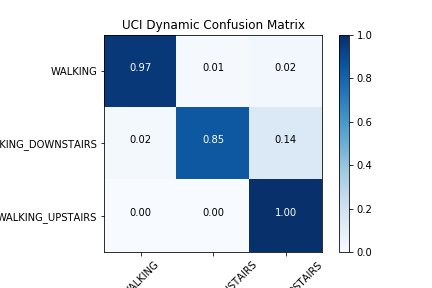
\includegraphics[width=.2\textwidth]{UCI_Dynamic_Confusion_Matrix}\hfill
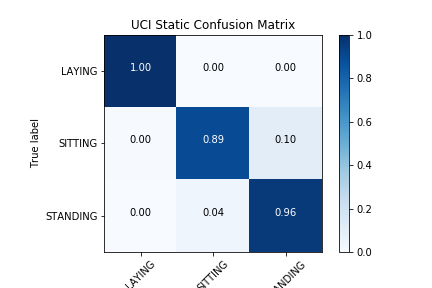
\includegraphics[width=.2\textwidth]{UCI_Static_Confusion_Matrix}\hfill
\caption*{Dynamic(left) and Static(right) UCI Model Confusion Matrices}
\label{UCI_Confusions}
\end{figure}

\subsubsection{UCI Dynamic \& Static}
These models achieved very high results (>90\%) however a little overfitting was observed.
To combat this overfitting, the epoch count was reduced however this started affecting general accuracy and so it was decided to keep epochs at 10 and accept a little overfitting.
It was also noted that although results where mostly consistent, each new run would change the overall accuracy score by 2\% on average.
The Static model achieved the highest results from the CNN models.
Due to their high accuracy, the f-score, precision and recall metrics resulted in similarly high results and offered little new information.

%\begin{figure}[h]
%\centering
%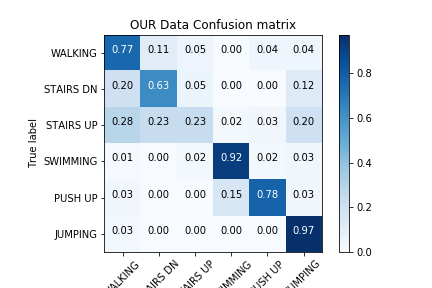
\includegraphics[width=.2\textwidth]{OD_Dynamic_Confusion_Matrix}\hfill
%\includegraphics[width=.2\textwidth]{OD_Static_Confusion_Matri}\hfill
%\caption*{Dynamic(left) and Static(right) OD Model Confusion Matrices}
%\label{OD_Confusions}
%\end{figure}

\subsubsection{Our Dataset Dynamic \& Static}
Initially the architecture for the UCI Dataset models would not function on our dataset.
It was found that the activation function of the last fully connected layer had to be changed from Softmax to LogSoftmax.
This affected the performance of the models as it increased the processing load.
The Dynamic model achieved good results with an accuracy of more than 60\%, when considering it trained on a reduced sized dataset with an equal distribution of 15\% for each label.
The extra effort put in to balance out the training distribution was expected to benefit the model in terms of accuracy, however there was no difference between the results of the model before the data balancing and after.
The higher precision score of 71\% compared to the recall of 61\% shows that the model is still able to predict the relevant label.
The Static model achieved very high results (more than 90\%).
The same steps taken for the UCI dynamic \& static models where taken and decided upon.



